\chapter{The Integrated System}
\label{chapter5}
Throughout the methods being developed and tested, they had to be added and integrated together into an overall system. This chapter describes the process taken to integrate all of the features together by using service communications, roslaunch files and basic logic to create the final product.
\section{Feature Integration}
After the features had been developed from the Methods section, a major challenge was to integrate all of these features to work together in the shop environment. This was done by first moving the code from all the manipulation tasks into one file\footnote{Github repository: Manipulation - shopkeeper.py. \url{https://github.com/um10kh/baxter-project/blob/master/src/manipulation/src/robot_shopkeeper_nk.py}} to allow the shopkeeper to be able to do all the manual tasks required. These manual tasks were commented clearly and placed under the \textit{Shopkeeper} class.
\newline\newline
Once, Baxter was able to carry out the manual tasks such as tilting the bowl and grabbing sweets, the next task was to integrate a communications system (using the \textit{Communications} class), to connect the main Shopkeeper node with the vision/other nodes. The main method of doing this was with custom service messages, where the Shopkeeper node would launch a service, sending a custom message, using a .srv file structure. The Shopkeeper node would then wait for an appropriate response returned from another node, before retrieving the information and using it. An example of this would be when Baxter was waiting for a customer to appear. He would look where he expected a customer then send the \textit{find\_person} node a message to find the next customer. That node would then wait for a customer to approach Baxter and wait in front of the camera, before sending a confirmation message back to the main node. This principle was used on the other aspects of the system too, such as finding the bowl, finding the sweets on the table and receiving voice commands from the Android application.
\subsection{Roslaunch Files}
Once all of the code and communications had been integrated into one file, a roslaunch file\footnote{Github repository - Launch - shopkeeper.launch. \url{https://github.com/um10kh/baxter-project/blob/master/src/manipulation/launch/shopkeeper.launch}} was built to help make the setup of the software more simple. Without a roslaunch file, the system had to be run by starting specific nodes at specific times, with around 9 different terminals running at the same time. The idea of this file was for there to only be one command to launch them all at the appropriate time, for ease of setup and testing. The basic approach would first launch all of the main Baxter-related nodes such as tucking his arms (so they always start in a fixed position) and opening the right hand camera and head camera with their correct resolutions. Then, the main vision systems were started, looking for the sweet area, the bowl on the table and the customer entry. After that, the application server would be started on the node and the application on the device, meaning the main shopkeeper node could then be run.
\subsection{System Logic}
The roslaunch file meant that all the nodes could run at once however, to make the manipulation and vision tasks fully integrated, some system logic was developed for Baxter to be able to constantly run these nodes, looking for new customers and running the `shop' more intelligently.
\begin{figure}[H]
        \centering 
        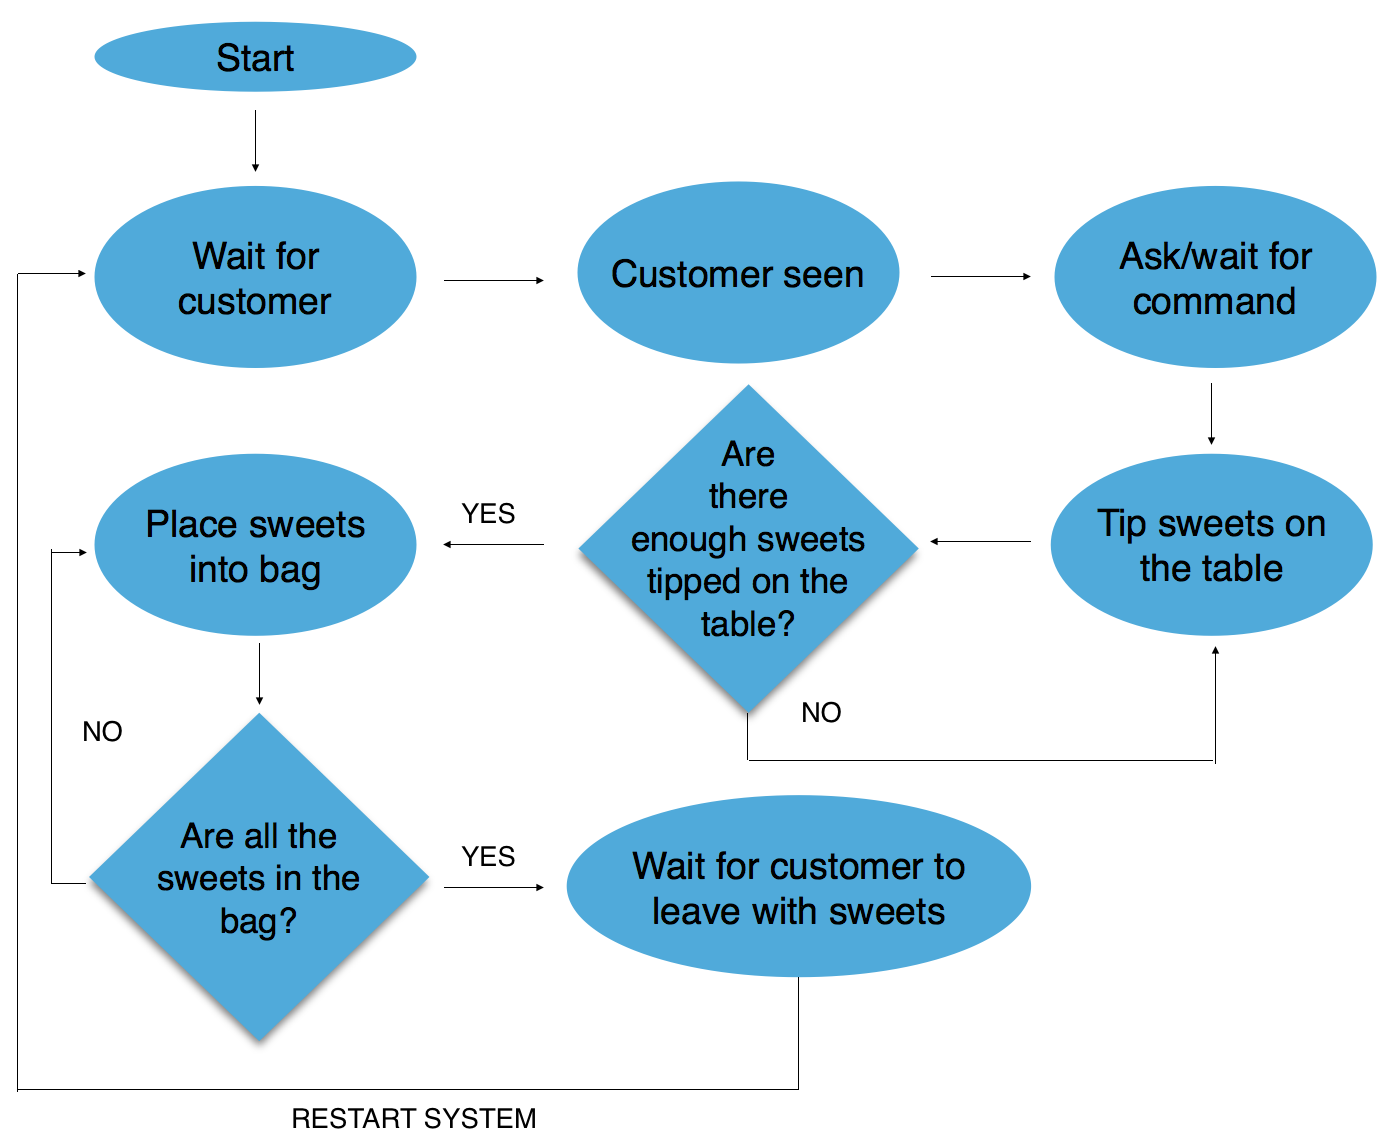
\includegraphics[width=0.75\textwidth, height=10cm]{completesystemlogic.png}
        \caption{A flow chart showing the overall system logic used to build the integrated system.}
         \label{fig:fakegripper}
\end{figure}
The key way to implement the logic was to develop the code around the major decision points. The basic way to do this was to implement while loops with logic checks. For example, a while loop would start, checking the sweets on the table using the sweet vision system. Then if there weren't enough sweets, Baxter would keep looping the code,  tipping the bowl continually onto the table until there were enough sweets, which would  break out of the loop. This principle was used for all the major decision points in the logic system and a `while True' loop was placed round the whole system so once a customer had left, the whole system would start again.
\subsection{User Setup}
Once the logic was implemented and the roslaunch file was written, setup options were added to the start of the program to make it easier for the user to start the system. Since there was no bag/sweet container recognition developed, I implemented a setup function that would prompt the user to place the right arm over the sweet bag and press enter, saving the joint positions so Baxter knew where to drop the sweets. Other user prompts for user setup were made in the same way. The user was prompted to open the android app and enter the shared IP address from the terminal and to place the gripper onto the table to retrieve the table's z height.
\newline\newline
An issue that arose towards the end of the system was when Baxter tried to grab some sweets, the inverse kinematics system caused his arm to knock off and break the clamp/stand for the Kinect attached to his torso. To get by this, a roslaunch file was created to ignore the bowl detection nodes and the user setup prompted the user to move the bowl underneath Baxter's gripper. This helped to test the overall system without having to use the Kinect. The user setup README\footnote{Github repository: User README. \url{https://github.com/um10kh/baxter-project/blob/master/README.md}} explains how the user could setup the system with or without the use of a Kinect.
\section{Integrated System Images}
Once the integration had been implemented along with the user setup, it was then time to test the final system. Firstly, a video taken to demonstrate the capabilities of the system. Stills from this video\footnote{Github repository - Complete System Video. \url{https://github.com/um10kh/baxter-project/blob/master/videos/IntegratedSystemCompressed.mp4}} are provided below in \textbf{\Cref{fig:completeSystem}} and show from (a) to (i) how a generic customer-shopkeeper transaction takes place with Baxter.\newline\newline
In this particular scenario, the customer approaches Baxter and when prompted, asks for one blue, one red and one green sweet. On his first attempt, he tips out the sweets, recognises them and grasps them from the small pile on the left of the page.
\begin{figure}[H]
\makebox[\linewidth][c]{%
\begin{subfigure}[b]{.43\textwidth}
\centering
\caption{}
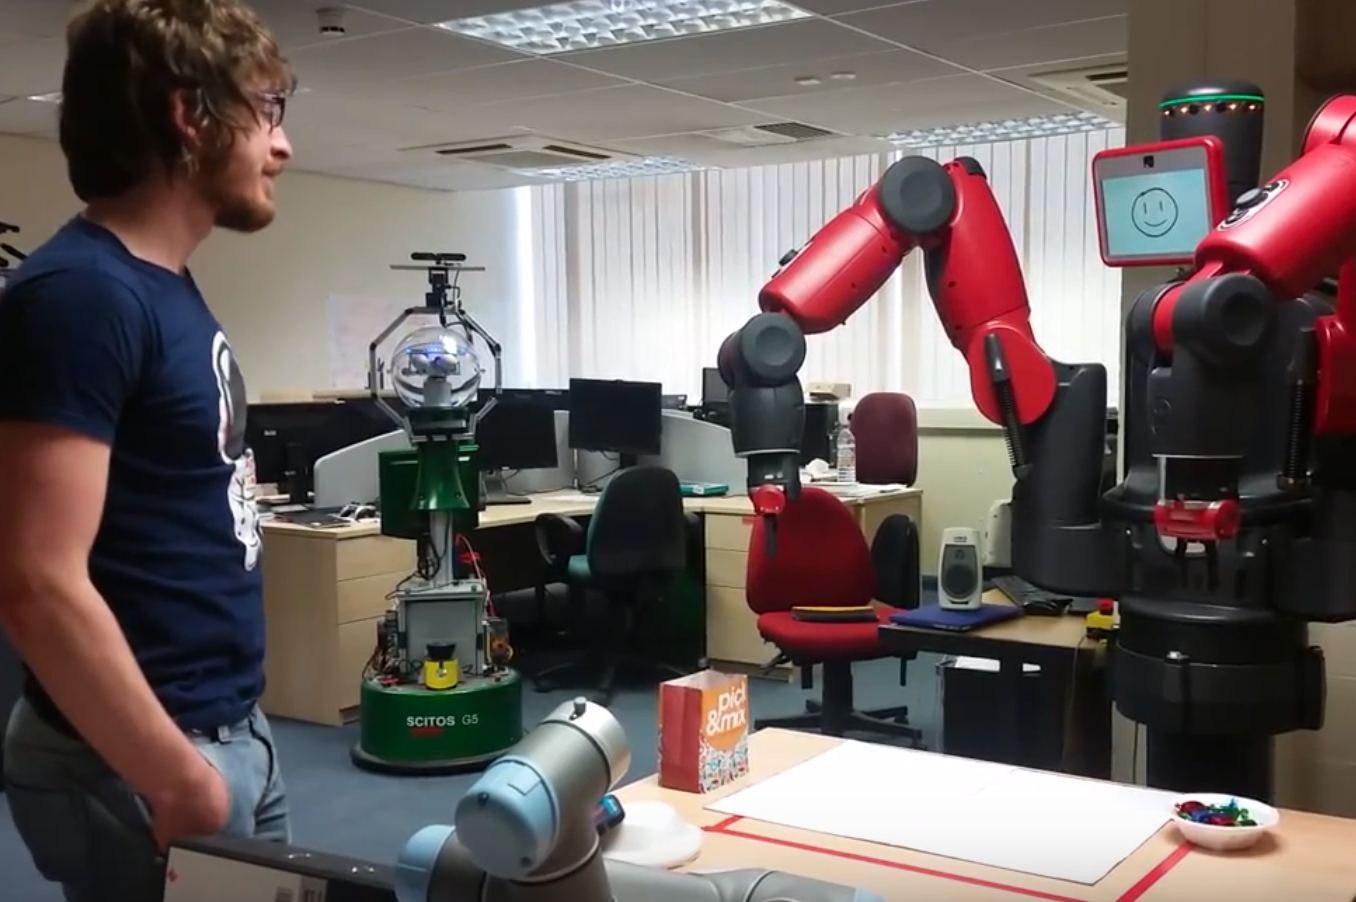
\includegraphics[width=.95\textwidth, height=4.3cm]{1.png}
\end{subfigure}%
\begin{subfigure}[b]{.43\textwidth}
\centering
\caption{}
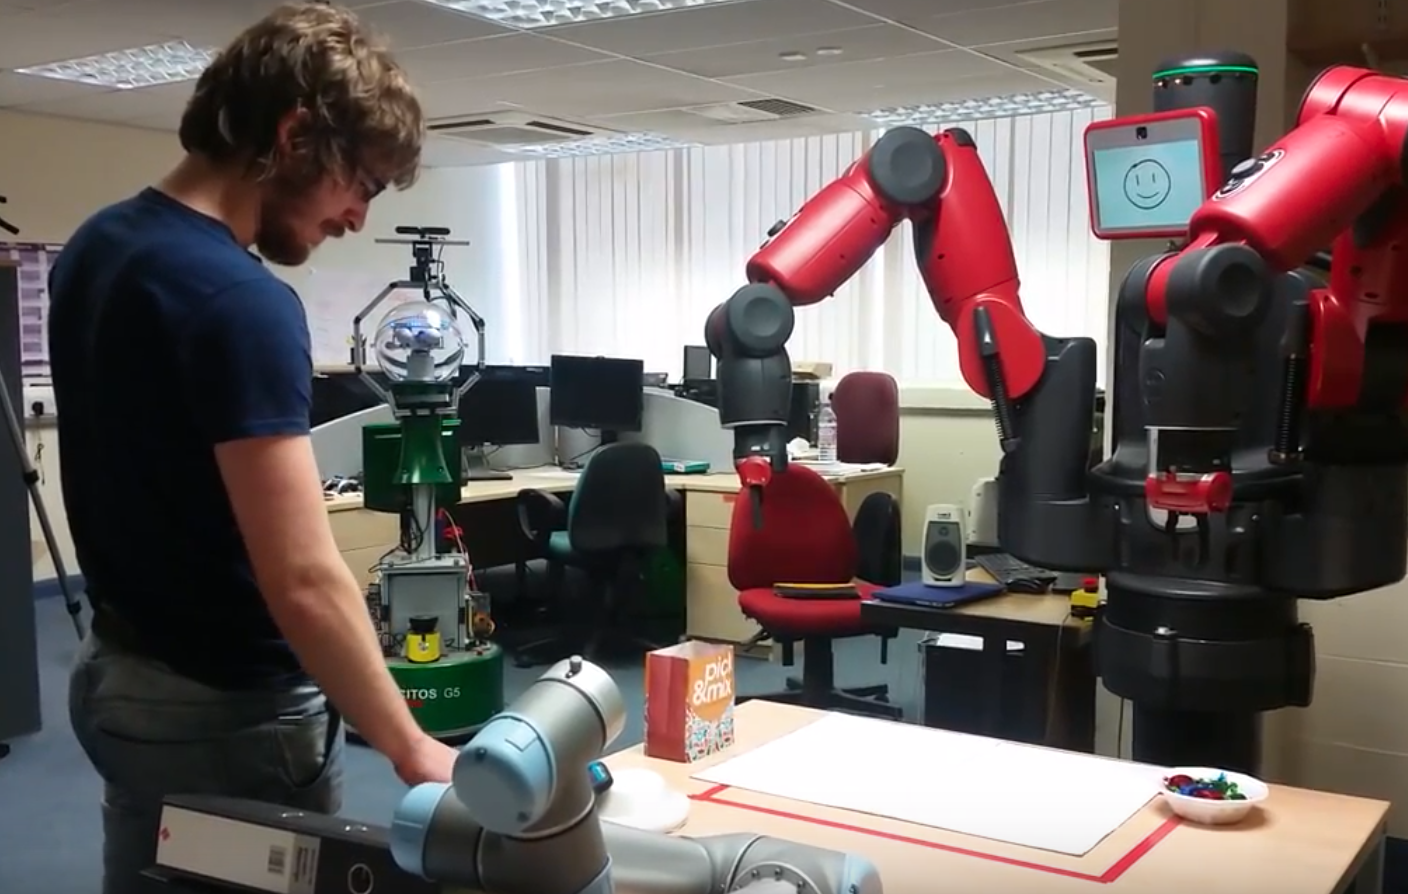
\includegraphics[width=.95\textwidth, height=4.3cm]{3.png}
\end{subfigure}%
\begin{subfigure}[b]{.43\textwidth}
\centering
\caption{}
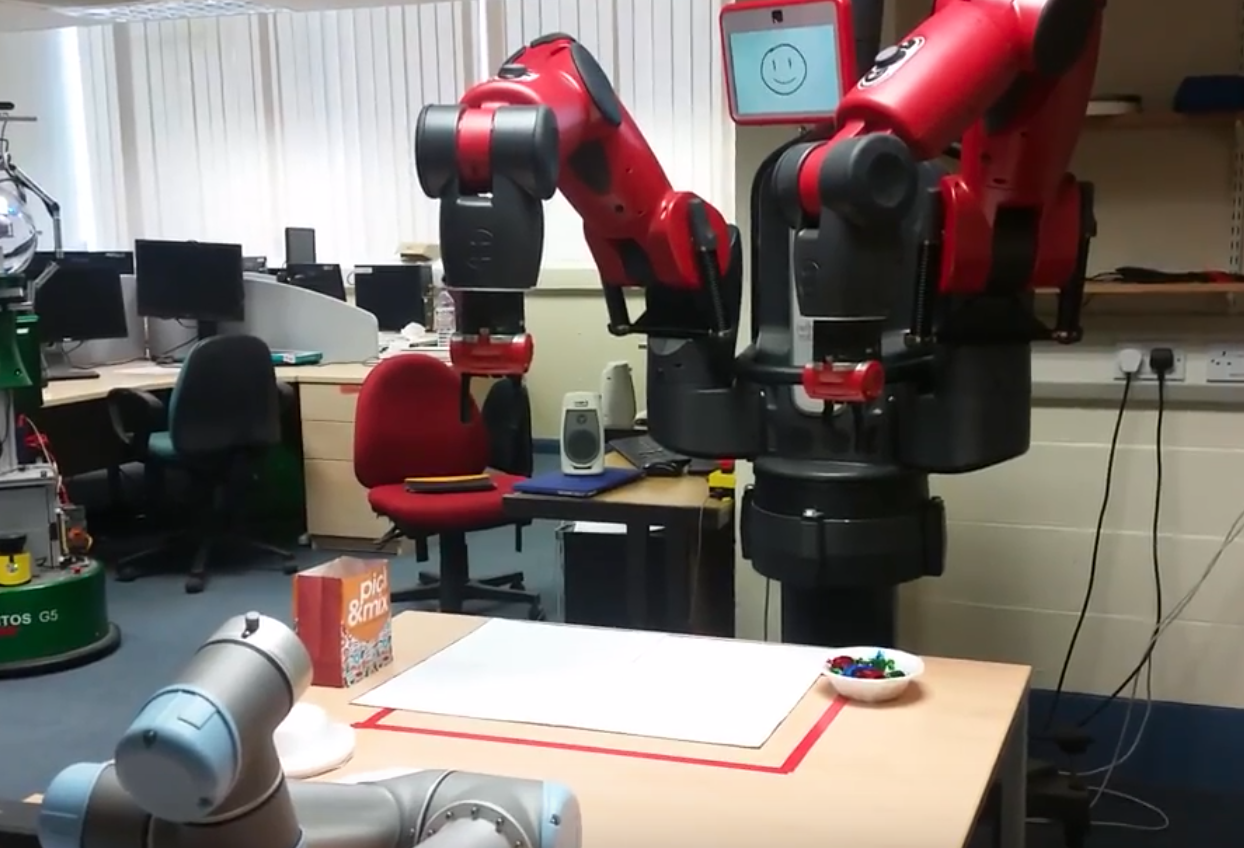
\includegraphics[width=.95\textwidth, height=4.3cm]{4.png}
\end{subfigure}%
}\\
\makebox[\linewidth][c]{%
\begin{subfigure}[b]{.43\textwidth}
\centering
\caption{}
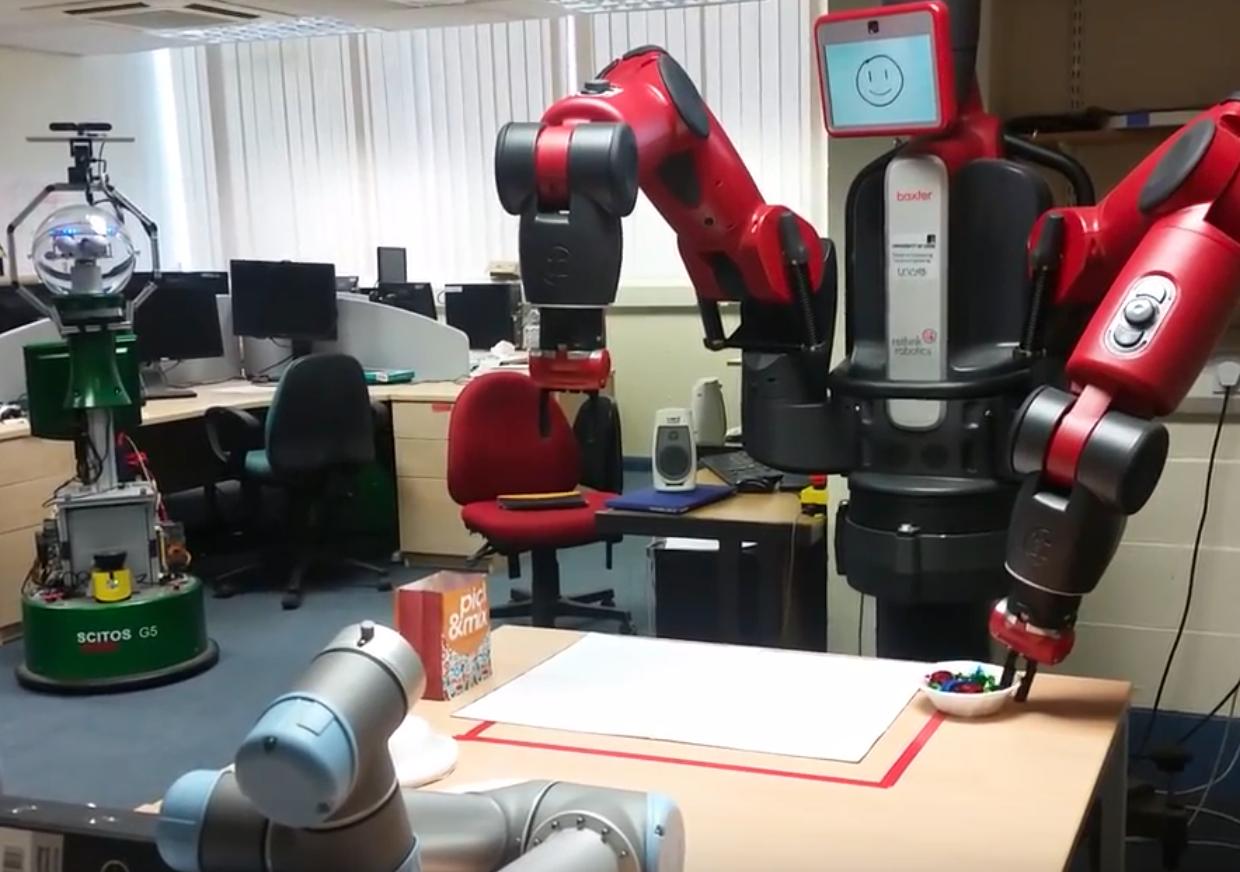
\includegraphics[width=.95\textwidth, height=4.3cm]{5.png}
\end{subfigure}%
\begin{subfigure}[b]{.43\textwidth}
\centering
\caption{}
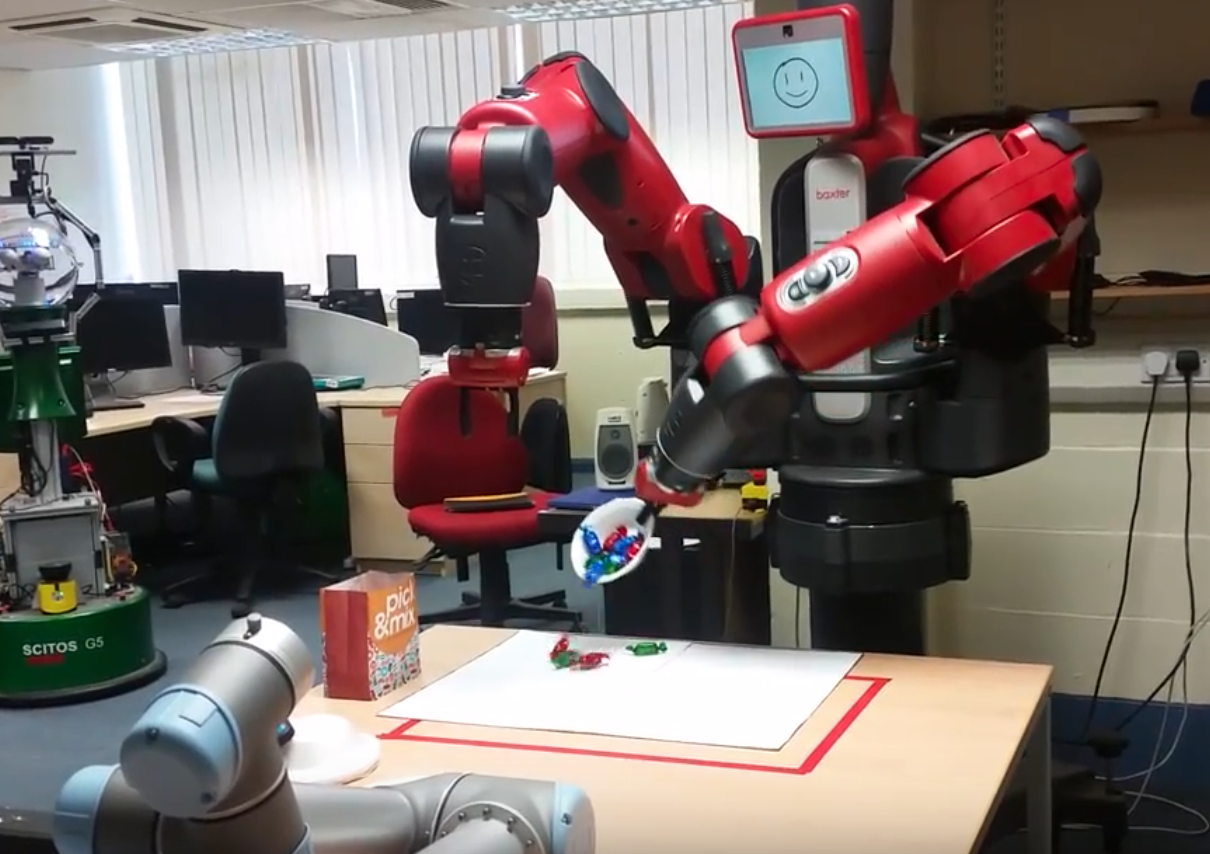
\includegraphics[width=.95\textwidth, height=4.3cm]{7.png}
\end{subfigure}%
\begin{subfigure}[b]{.43\textwidth}
\centering
\caption{}
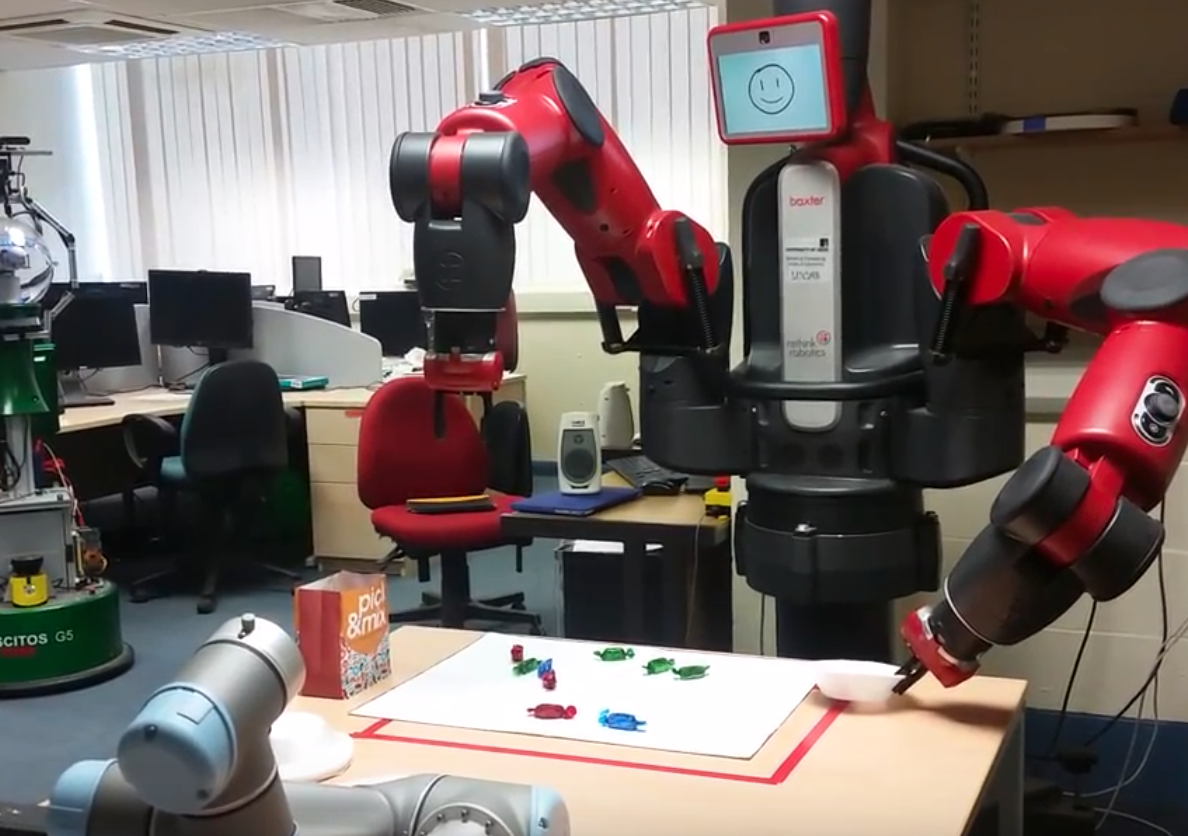
\includegraphics[width=.95\textwidth, height=4.3cm]{8.png}
\end{subfigure}%
}\\
\makebox[\linewidth][c]{%
\begin{subfigure}[b]{.43\textwidth}
\centering
\caption{}
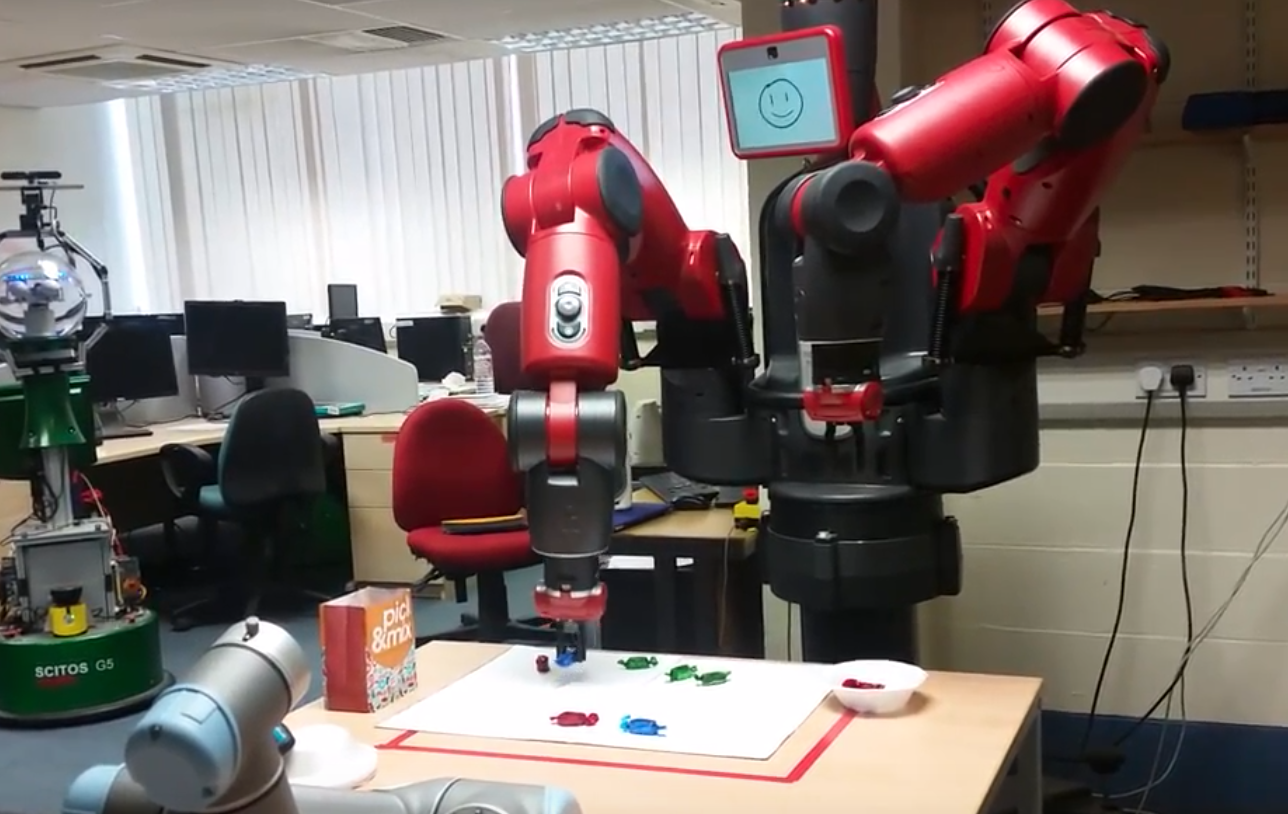
\includegraphics[width=.95\textwidth, height=4.3cm]{11.png}
\end{subfigure}%
\begin{subfigure}[b]{.43\textwidth}
\centering
\caption{}
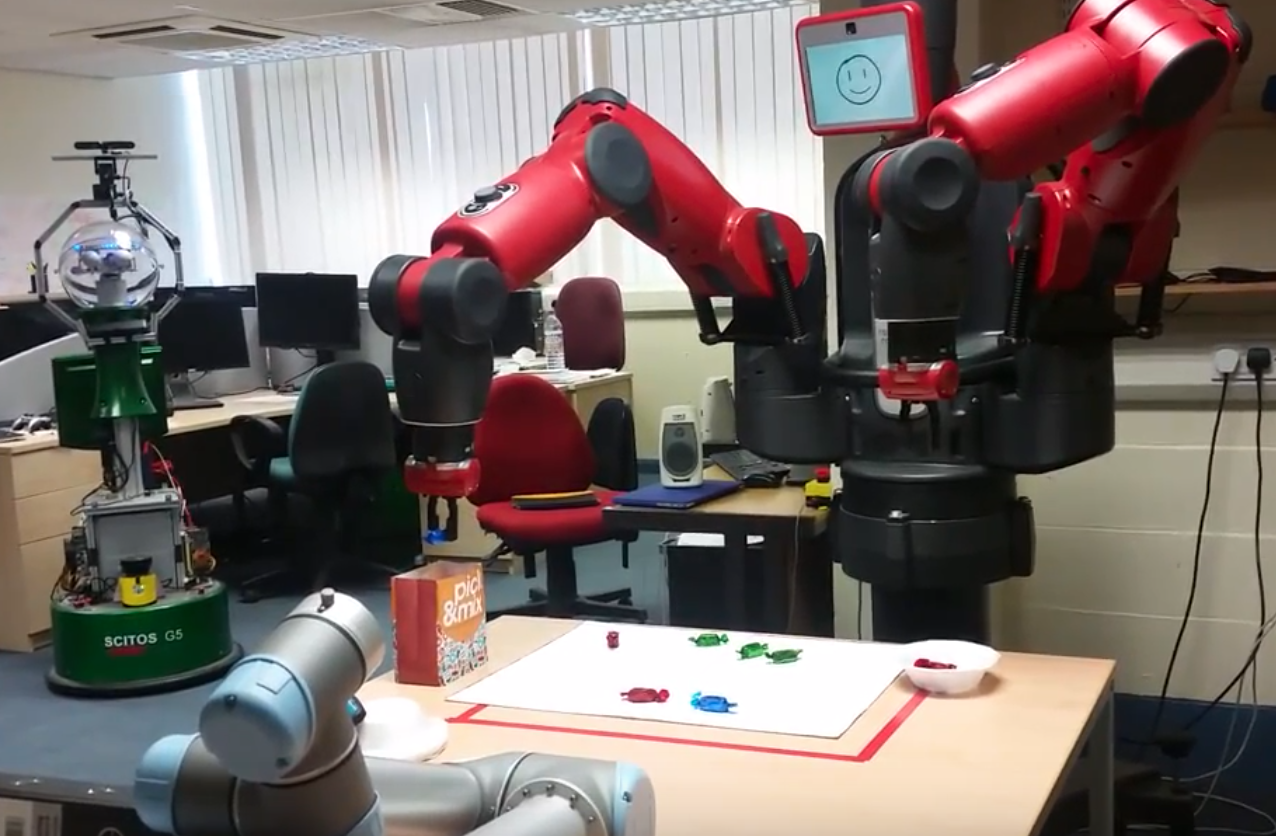
\includegraphics[width=.95\textwidth, height=4.3cm]{12.png}
\end{subfigure}%
\begin{subfigure}[b]{.43\textwidth}
\centering
\caption{}
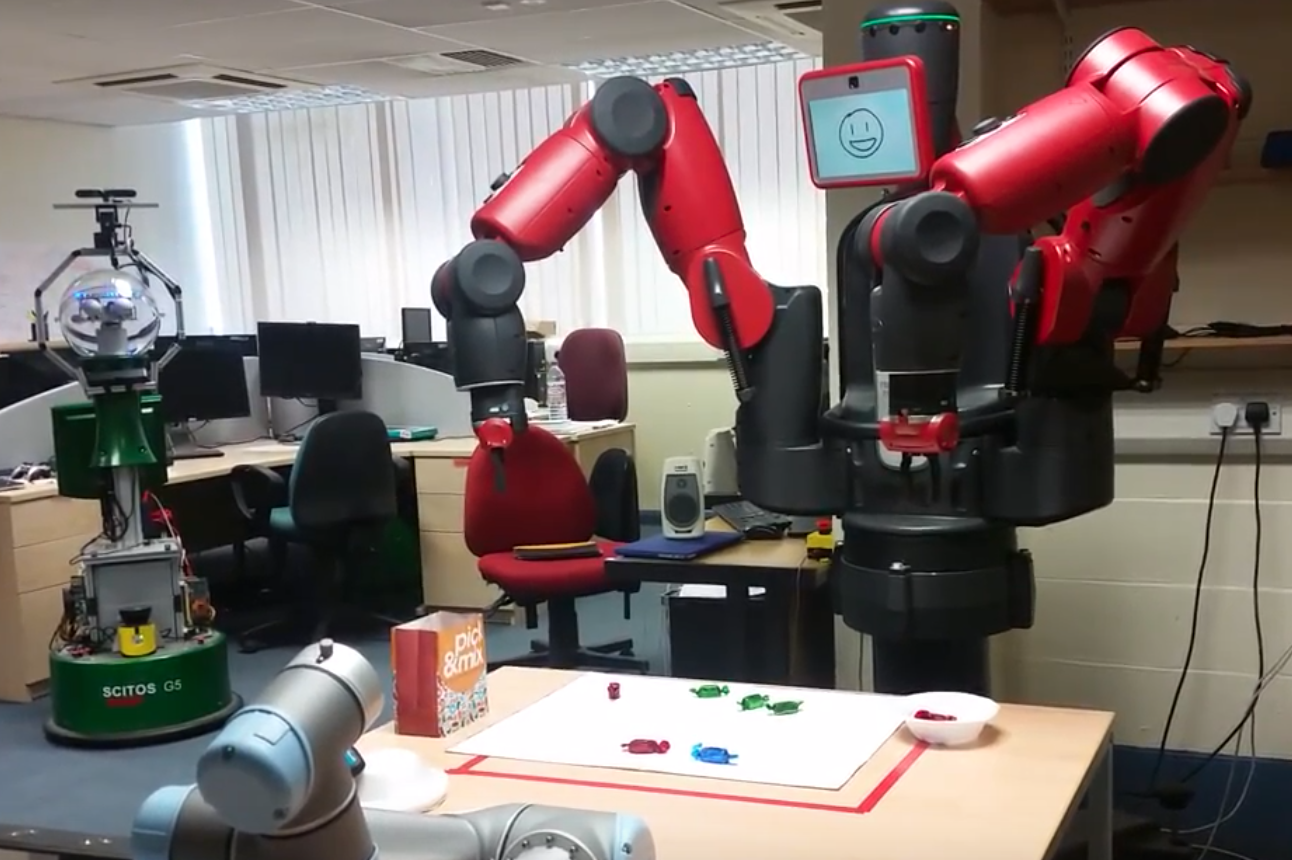
\includegraphics[width=.95\textwidth, height=4.3cm]{13.png}
\end{subfigure}%
}
\caption{An example of the complete working system: (a) Baxter recognises the customer and asks them to provide a voice command for their sweets. (b) The customer says how many blue, red and green sweets they want and confirms on the Android app. (c) Baxter checks the table to make sure there aren't enough sweets on the table already. (d) He looks for the bowl and goes to grab it. (e) The bowl is tipped in two locations above the page. (f) The sweets on the table are scanned, counted and analysed. (g) The requested sweets are grabbed from the table. (h) The grabbed sweets are placed into the sweet bag. (i) Baxter has completed his request, thanks the customer and waits for the next one.}
\label{fig:completeSystem}
\end{figure}
\section{Evaluating the System}
To test the overall system, five different human customers were asked to walk up to Baxter and order some sweets. The reliability of the system was judged on multiple levels: on whether Baxter understood the command, on whether he correctly placed the requested sweets in the bag and on the customer satisfaction with the ease of the process. After doing the human tests, a few observations were made below on the problems encountered.
\newline\newline
Variations in voice/accents provided difficulty for the voice recognition system (although that was expected and more a limitation of the device than the software). Sometimes the voice recognition didn't recognise the colour stated, leaving the rest to be unrecognised too. With more time, multiple accents could be trialled and an increasingly wider search of terms could be accepted for the colours to correct this. Tipping the sweets onto the table, whilst reasonably reliable at separating the sweets, the tilting method still managed to produce hard-to-separate sweet piles. It tended to depend on how the sweets were placed in the bowl initially. As long as the colours and orientations were mixed it seemed OK however, if they were all bunched together in colour order, all facing the same way, a lot of sweets could be tipped out at once. Since the addition of the speech to Baxter, the customers found the interaction reasonably simple to carry out. The face letting the customer know when they were recognised also helped (in case of a slightly inaccurate detection and the customer needed to move about a bit more).
\newline\newline
The trials overall, even after multiple customers had approached Baxter, were very good on the whole, and reliable enough that if Baxter did make a mistake, he knew about it and could correct it. If he missed grabbing a sweet, he would try to grab another, if he hadn't tipped enough sweets on the table to recognise, he would continue tipping until there were enough. Occasionally Baxter grabbed two sweets from a pile instead of one and gave them slightly more than they ordered but that wasn't a important issue. The main issues were on the setup of the system (either the TTS or app server had an issue in starting), but after a reboot of the roslaunch file, the system tended to work well again. 
\section{Limitations/Improvements}
Overall, whilst most of the actions in the shop had been tested to determine reliability, there were still some issues that existed by the end of the project. Here, I will discuss the issues and limitations demonstrated by the final version of the system and approaches I would like to take to these problems if I would have had more time to do so.\newline\newline
\textbf{Human interaction}\newline
The problem with the final interaction system was that there were some gaps in the conversation and interaction that made it not seem lifelike. The main improvements that could have been made with more time were to use a proper skeleton recognition system, so Baxter could constantly recognise the person's skeleton and perform gesture recognition. I feel like the ability for the customer to exchange items with Baxter, such as exchange money or take the bag of sweets would have added to the realism of the interaction greatly. Another issue that was mentioned was to implement threading and idle movements. Threading would have helped Baxter move both arms together in more human-like movements (instead of moving them one at a time). Idle movements were discussed as an addition to make Baxter seem lifelike even when he was not talking to a customer. As future tasks, it would be nice for those to be implemented so at the open day, Baxter would not be stood still until a customer approached him.
\newline\newline
\textbf{Sweet Recognition}\newline
Whilst this system was reasonably reliable by the end (and a lot more efficient than it was in initial iterations), there were still some problems that needed to be rectified. To be more robust, the sweet recognition system should have been made to work within different shop-like settings. The problem was different light sources would affect the testing data used to train the neural network. Therefore if the shop had a different coloured light source, the sweet colour recognition would be unreliable. I think a good way to solve this problem would be to add a user setup method to train new sweets under new conditions and automate the process. That would mean a user could then run the software, place multiple target sweets onto the table and Baxter would record their data and train the neural network. That addition to the system would certainly make it easier and more robust to be used in different rooms throughout the university for open days.\newline\newline
\textbf{Sweet Singulation}\newline
If there was more time, a more efficient sweet singulation algorithm would be proposed/developed. The problem with singulating the sweets vision-wise and manipulation-wise is that there was no clear way to do this task. I carried out a lot of research and there is no specified way to be able to recognise individual, deformable objects within a cluster, with variable shape and colour. The fact that the sweets could vary in shape so much, meant that most vision techniques using shape recognition would not work - for example, template matching was considered but it could not be reliably implemented. The variation in colour meant that the sweets could not be differentiated easily by colour as all three wrapper colours could overlap in the HSV or RGB colourspace. Therefore, the combined method I used, using colour detection, then other processing methods was the best method I could manage to implement, but with more time, I think there would be a more accurate, computationally efficient approach to solve this.
\section{Project Reflection}
Over the past twelve weeks, I have really enjoyed this project and I think that mainly, it went very well and I am pleased with the overall deliverables produced. The main problem I think I had was organisation of time. After doing the initial planning report and the supervisor/assessor presentation at week 8, the main issues with the feedback from both those meetings were that the time limit was overly ambitious and at some point, some features would have to be cut out. By the end of the project, there were multiple discussed parts of the project that were not developed: money exchange with the customer and fully developed sweet singulation were some of the key features that I didn't have time to complete. Whilst money exchange with the customer was a stretch goal anyway, the sweet singulation methods turned out to be a lot more of a complex issue than initially proposed.
\newline\newline
If I were to do the project again, I think I would have started coding and work on the project earlier. A major issue was that I started developing the bowl recognition system with the Kinect as the first task. It took a long time to get used to the methods and PCL libraries. The problem was that the first main coding task was based on two completely new pieces of software: ROS and the PCL library. I feel that if I had started with the simpler OpenCV/Python based coding tasks first, it would've made the project easier to start and develop and could have prevented getting stuck for as long in the initial few weeks. Possibly the reason why the bowl recognition task took so long is because ROS was quite difficult to pick up and use and there wasn't a lot of great documentation out there to explain the core concepts of it. Once I got to around week 6, I felt like I fully understood the principles of ROS and could therefore do a lot more with it.
\newline\newline
Looking back at the initial objectives, they stated I needed to develop a vision system for the bowl, sweets, a manipulation system for them and a some human interaction systems. I believe that I have achieved all of these basic objectives to some extent and am very happy with the quality of the results produced at each stage. I thoroughly enjoyed the overall project and feel like I got a lot out of it. The weekly meetings with my supervisor were very useful, to discuss and develop ideas with but mainly, I feel a sense of achievement that I mainly developed this entire project on my own.